\section{The coordinate system}

These macros replace those of \tkzname{tkz-base} (\tkzcname{tkzInit}, \tkzcname{tkzGrid}, \tkzcname{tkzAxeXY}, \tkzcname{tkzDrawX}, \tkzcname{tkzClip}, \tkzcname{tkzRep}, \tkzcname{tkzText}).

\subsection{Initialization: \tkzcname{tkzFnInit}}

\begin{NewMacroBox}{tkzFnInit}{\oarg{options}}
\begin{tabular}{lll}
\toprule
options             & default & definition  \\
\midrule
\TOline{xmin}{-5}{smallest $x$}
\TOline{xmax}{5}{largest $x$}
\TOline{xstep}{1}{value represented by 1 cm on the $x$-axis}
\TOline{ymin}{-5}{smallest $y$}
\TOline{ymax}{5}{largest $y$}
\TOline{ystep}{1}{value represented by 1 cm on the $y$-axis}
\TOline{xorigin}{0}{$x$ placed at $X=0$ (a year, for example)}
\TOline{yorigin}{0}{$y$ placed at $Y=0$}
\TOline{enlarge}{0 (0.1 without value)}{enlarges the window by a fraction of its size}
\TOline{enlarge x, enlarge y}{enlarge}{enlargement in one direction only}
\bottomrule
\end{tabular}

\emph{Values can be expressions: \texttt{xmax=2*pi}.}
\end{NewMacroBox}

\subsection{Grid: \tkzcname{tkzFnGrid}}

\begin{NewMacroBox}{tkzFnGrid}{\oarg{options}\parg{$x_1$,$y_1$}\parg{$x_2$,$y_2$}}
\emph{The region is optional; by default the grid covers the window.}

\begin{tabular}{lll}
\toprule
options             & default & definition  \\
\midrule
\TOline{dx}{xstep}{distance between two vertical lines}
\TOline{dy}{ystep}{distance between two horizontal lines}
\TOline{sub}{false}{adds a subgrid}
\TOline{subdx}{dx/5}{spacing of the subgrid}
\TOline{subdy}{dy/5}{spacing of the subgrid}
\bottomrule
\end{tabular}

\emph{Other options are \TIKZ\ options; the style is \tkzname{tkzfn grid}.}
\end{NewMacroBox}

\begin{tkzexample}[latex=8cm]
\begin{tikzpicture}[scale=1.25]
 \tkzFnInit[xmin=-2,xmax=3,
            ymin=-1,ymax=2]
 \tkzFnGrid[sub,color=orange]
 \tkzFnAxes
\end{tikzpicture}
\end{tkzexample}

\subsection{Axes: \tkzcname{tkzFnAxes}, \tkzcname{tkzFnAxisX}, \tkzcname{tkzFnAxisY}}

\begin{NewMacroBox}{tkzFnAxes}{\oarg{options}}
\emph{Draws both axes, the tick marks and their labels. The axes cross at $(0, 0)$ if this point is in the window, at $(x_{\min}, y_{\min})$ otherwise. Values are written in the American or the French way (section~\ref{sec:format}).}

\begin{tabular}{lll}
\toprule
options             & default & definition  \\
\midrule
\TOline{dx, dy}{xstep, ystep}{distance between two tick marks}
\TOline{xlabel, ylabel}{\$x\$, \$y\$}{names of the axes}
\TOline{ticks}{true}{tick marks}
\TOline{labels}{true}{tick labels}
\TOline{line}{true}{axis lines}
\TOline{origin}{0 or O}{label of the origin (0 American, O French)}
\TOline{trig}{0}{if $n>0$, ticks of the $x$-axis at multiples of $\pi/n$}
\TOline{decimals}{4}{maximum number of decimal places}
\TOline{arrows}{end}{arrows: \texttt{end}, \texttt{both} or \texttt{none} (section~\ref{sec:arrows})}
\TOline{box}{false}{``box'' axes (section~\ref{sec:box})}
\TOline{style}{school}{\texttt{school} or \texttt{box}}
\TOline{tick length}{3pt}{length of the tick marks (box)}
\bottomrule
\end{tabular}

\emph{\tkzcname{tkzFnAxisX} and \tkzcname{tkzFnAxisY} draw a single axis; their options are the same with \tkzname{label}, \tkzname{label style} and \tkzname{step} instead of \tkzname{xlabel}, \tkzname{ylabel} and \tkzname{dx}. With \tkzname{ticks=false}, you get the equivalent of \tkzcname{tkzDrawX}.}
\end{NewMacroBox}

\begin{tkzexample}[latex=8cm]
\begin{tikzpicture}
  \tkzFnInit[xmin=-7,xmax=7,
             ymin=-1,ymax=1]
  \tkzFnAxisY
  \tkzFnAxisX[trig=2]
  \tkzFnDraw[red]{sin(x)}
\end{tikzpicture}
\end{tkzexample}

\subsection{Clipping: \tkzcname{tkzFnClip}}

\begin{NewMacroBox}{tkzFnClip}{\oarg{margin in pt}}
\emph{Restricts the rest of the drawing to the window (enlarged by a margin). As with \tkzcname{clip}, use it preferably inside a \tkzname{scope} environment. Curves and tangent lines are clipped to the window anyway (option \tkzname{clip}).}
\end{NewMacroBox}

\subsection{Unit vectors: \tkzcname{tkzFnRep}}

\begin{NewMacroBox}{tkzFnRep}{\oarg{\TIKZ\ options}}
\emph{Draws the vectors $\vec{\imath}$ and $\vec{\jmath}$; the style is \tkzname{tkzfn rep}.}
\end{NewMacroBox}

\subsection{Text: \tkzcname{tkzFnText}}

\begin{NewMacroBox}{tkzFnText}{\oarg{\TIKZ\ options}\parg{$x$,$y$}\marg{text}}
\emph{Places a text at the point with coordinates $(x, y)$ in the coordinate system. You can also give the name of a point: \tkzcname{tkzFnText}\texttt{[above](A)\{text\}}.}
\end{NewMacroBox}

\begin{tkzexample}[latex=8cm]
\begin{tikzpicture}[scale=1.5]
 \tkzFnInit[xmin=-3,xmax=3,
            ymin=-1,ymax=4]
 \tkzFnGrid[sub,subdx=.5,subdy=.5]
 \tkzFnAxes
 \tkzFnDraw[domain=-3:2]{(2-x)*exp(x)}
 \tkzFnText(-2,1.25){$\mathcal{C}_{f}$}
 \tkzFnRep
\end{tikzpicture}
\end{tkzexample}

\subsection{Arrows at both ends: \tkzname{arrows}}\label{sec:arrows}

In the United States, textbooks and graphing calculators often put an arrow at each end of the axes. The option \tkzname{arrows} of \tkzcname{tkzFnAxes}, \tkzcname{tkzFnAxisX} and \tkzcname{tkzFnAxisY} chooses the arrows:
\begin{itemize}
  \item \texttt{end} (default): one arrow at the positive end;
  \item \texttt{both}: an arrow at each end;
  \item \texttt{none}: no arrow.
\end{itemize}
|\tkzFnSetup{arrows=both}| chooses the arrows for all the following coordinate systems. The shape of the arrow tips is given by the style \tkzname{tkzfn axis}.

\begin{tkzexample}[latex=7cm]
\begin{tikzpicture}[scale=.6]
  \tkzFnInit[xmin=-5,xmax=5,
             ymin=-4,ymax=6]
  \tkzFnGrid
  \tkzFnAxes[arrows=both]
  \tkzFnDraw[blue,thick,<->,>=stealth,
             clip=false,domain=-4.2:4.2]{x^2/2-3}
\end{tikzpicture}
\end{tkzexample}

For a whole document, with other arrow tips:

\begin{tkzexample}[latex=7cm]
\tkzFnSetup{arrows=both}
\tikzset{tkzfn axis/.style={>=latex}}
\begin{tikzpicture}[scale=.7]
  \tkzFnInit[xmin=-2,xmax=3,xstep=.5,
             ymin=-1.5,ymax=1.5,ystep=.5]
  \tkzFnGrid[sub]
  \tkzFnAxes[dx=1]
  \tkzFnDraw[red,thick]{x^3/3-x}
\end{tikzpicture}
\tkzFnSetup{arrows=end}
\tikzset{tkzfn axis/.style={->,>=stealth}}
\end{tkzexample}

Without arrows:

\begin{tkzexample}[latex=7cm]
\begin{tikzpicture}[scale=.6]
  \tkzFnInit[xmin=-1,xmax=5,
             ymin=-1,ymax=3]
  \tkzFnAxes[arrows=none]
  \tkzFnDraw{sqrt(x)}
\end{tikzpicture}
\end{tkzexample}

\newpage
\subsection{``Box'' axes: \tkzname{box}}\label{sec:box}

This presentation is usual in scientific publications and with \tkzname{pgfplots}, and less common in high school textbooks. With \tkzname{pgfplots} it is obtained with the \tkzname{axis} environment; with \tkzname{tkz-fn} an option is enough:

\begin{itemize}
  \item |\tkzFnAxes[box]|: a frame surrounds the window, the tick marks point inward on the four sides, every value (including those at the edges) is written outside, there is no arrow and no origin label;
  \item the names of the axes are written only when they are given: |xlabel| below the frame, |ylabel| on the left, vertically;
  \item |\tkzFnSetup{axes=box}| chooses this presentation for all the following coordinate systems; |\tkzFnSetup{axes=school}| comes back to the usual one;
  \item the option \tkzname{mark} of \tkzcname{tkzFnDraw} puts a mark at each computed point (\tkzname{samples} sets their number);
  \item the option \tkzname{enlarge} of \tkzcname{tkzFnInit} moves the curve away from the frame; the default domain is still $[x_{\min}, x_{\max}]$.
\end{itemize}

The style of the frame is \tkzname{tkzfn box}. The following examples reproduce a figure made with \tkzname{pgfplots}.

\begin{tkzexample}[latex=7cm]
\tkzFnDef{f}{1/((1e9*x/11.778)*3.273e-8
              -3.273e-8+1)}
\begin{tikzpicture}[scale=.9]
  \tkzFnInit[xmin=0,xmax=6,
             ymin=0,ymax=1,ystep=.2]
  \tkzFnAxes[box]
  \tkzFnDraw[blue,mark=*,mark size=1.5pt,
             samples=13,domain=0:5](f)
  \tkzFnDrawData[red,mark=square*,
                 mark size=1.5pt]{.125/.744}
\end{tikzpicture}
\end{tkzexample}

The default domain is $[x_{\min}, x_{\max}]$:

\begin{tkzexample}[latex=7cm]
\begin{tikzpicture}[scale=.9]
  \tkzFnInit[xmin=0,xmax=6,
             ymin=0,ymax=1,ystep=.2]
  \tkzFnAxes[box]
  \tkzFnDraw[blue,mark=*,mark size=1.5pt,
             samples=25](f)
  \tkzFnDrawData[red,mark=square*,
                 mark size=1.5pt]{.125/.744}
\end{tikzpicture}
\end{tkzexample}

With \tkzname{enlarge} (10\,\% by default) and the names of the axes:

\begin{tkzexample}[latex=7cm]
\begin{tikzpicture}[scale=.9]
  \tkzFnInit[xmin=0,xmax=6,ymin=0,ymax=1,
             ystep=.2,enlarge]
  \tkzFnAxes[box,xlabel=$x$,
             ylabel=$f(x)$]
  \tkzFnDraw[blue,mark=*,mark size=1.5pt,
             samples=25](f)
  \tkzFnDrawData[red,mark=square*,
                 mark size=1.5pt]{.125/.744}
\end{tikzpicture}
\end{tkzexample}

\newpage
With |\tkzFnSetup{axes=box}|, the grid and the ticks at multiples of $\pi$ are used as usual; the option \tkzname{smooth} is passed to \TIKZ.

\begin{tkzexample}[vbox]
\tkzFnSetup{axes=box}
\begin{tikzpicture}[scale=.6]
  \tkzFnInit[xmin=-3,xmax=3,ymin=0,ymax=20000,ystep=4000]
  \tkzFnGrid
  \tkzFnAxes[xlabel=$t$,ylabel=Population]
  \tkzFnDraw[red,thick,smooth,samples=7]{2000*x^2}
\end{tikzpicture}\qquad
\begin{tikzpicture}[scale=.6]
  \tkzFnInit[xmin=-7,xmax=7,ymin=-1,ymax=1,ystep=.5]
  \tkzFnAxes[trig=2]
  \tkzFnDraw{sin(x)}
\end{tikzpicture}
\tkzFnSetup{axes=school}
\end{tkzexample}

\endinput
